\section{ECS Literature Review}

Historically, realtime interactive systems like simulations and game development have relied on object-oriented design techniques which introduced massive class hiearchies, deep inheritance paths, and highly specialized code to projects. The aim of an ECS is to allievate, or downright remove, many of the negatives that come with classical object-oriented design. ECS architectures follow the composition over inheritance principle, which aims to manage entities in large scale real-time applications efficiently. \cite{Haerkoenen2019} 

\subsection{Entity Component System Foundations}
These are the foundational definitions used in this paper.

\begin{tdefn}[Entity]
    An entity is a unique identifier used to represent a "thing" in the simulation. This unique identifier is used in some manner by the ECS to collect a set of components. Some ECS's try to make the identifier intelligent to optimize component selection by using the bytes in an integer to store more location information. This will be discussed in the existing ECS implementions.
\end{tdefn}
\begin{tdefn}[Component]
    Generally speaking, a component is data. It can be defined as a struct, tuple, or class. For this thesis, we define a component to only be a segment of either complete or incomplete data.
\end{tdefn}
\begin{tdefn}[Tag]
    A tag is a component such that it contains 0 information other than its existence.
\end{tdefn}
\begin{tdefn}[System]
    A system has two parts. First the query and second the execution. A system queries for a collection of components and then executes a function that can modifies, create, or destroy entities or components.
\end{tdefn}
\noindent The paper will build upon these four concepts and introduce new definitions based on these.

\subsection{The Weaknessess Of Object Oriented Programming}

% TODO: Sources
It has been exhaustively shown that Object-Oriented Programming (OOP) increases the difficulty of achieving desired simulation goals and that there are plenty attractive alternatives. The two main weaknesses that an ECS intends to solve is: poor cache utilization and poor parallelization.

Large projects deep into using OOP principles learn how hard it is to keep cached what you need and keep junk out. OOP principles can make pointer abuse very easy and cause the cache to overwrite potentially useful data in the near future. ECS solves this by introducing components. Since components are detached from their entity, we as engine designers can put these components wherever we please. It's not an uncommon practice to see component data be stored in long homogenous vectors. Suppose you have to do a heavy operation across the set of entities that all contain component $Q$. An ECS in this situation will be extremely cache friendly, due to $Q$ being next to components that all contain the same component type.

In OOP, parallelism can be painful due to synchronization errors over memory that was not engineered to effectively be parallelized. ECS follows principles from another design pattern called Data-Oriented Design (DOD). DOD, as a design theory, generally produces code that is more easily parallelizable. The concept of storing components as homogenous vectors not only helps with caching but because all data pertaining to a component is already in a homogenous vector -- it's easy to process in parallel or in groups.

\subsection{An Entity-Component System Model}

% TODO: NOTE, each thread gets a copy of this vector and we merge them at the first linearization point (next frame)
ECS Architectures are built upon two core data structures: vectors and hashmaps. The following architecture given is my naive ECS version. This example will not be thread safe and is purely for getting a taste of how different pieces of an ECS fit together.

\begin{figure}[htbp]
    \centering
    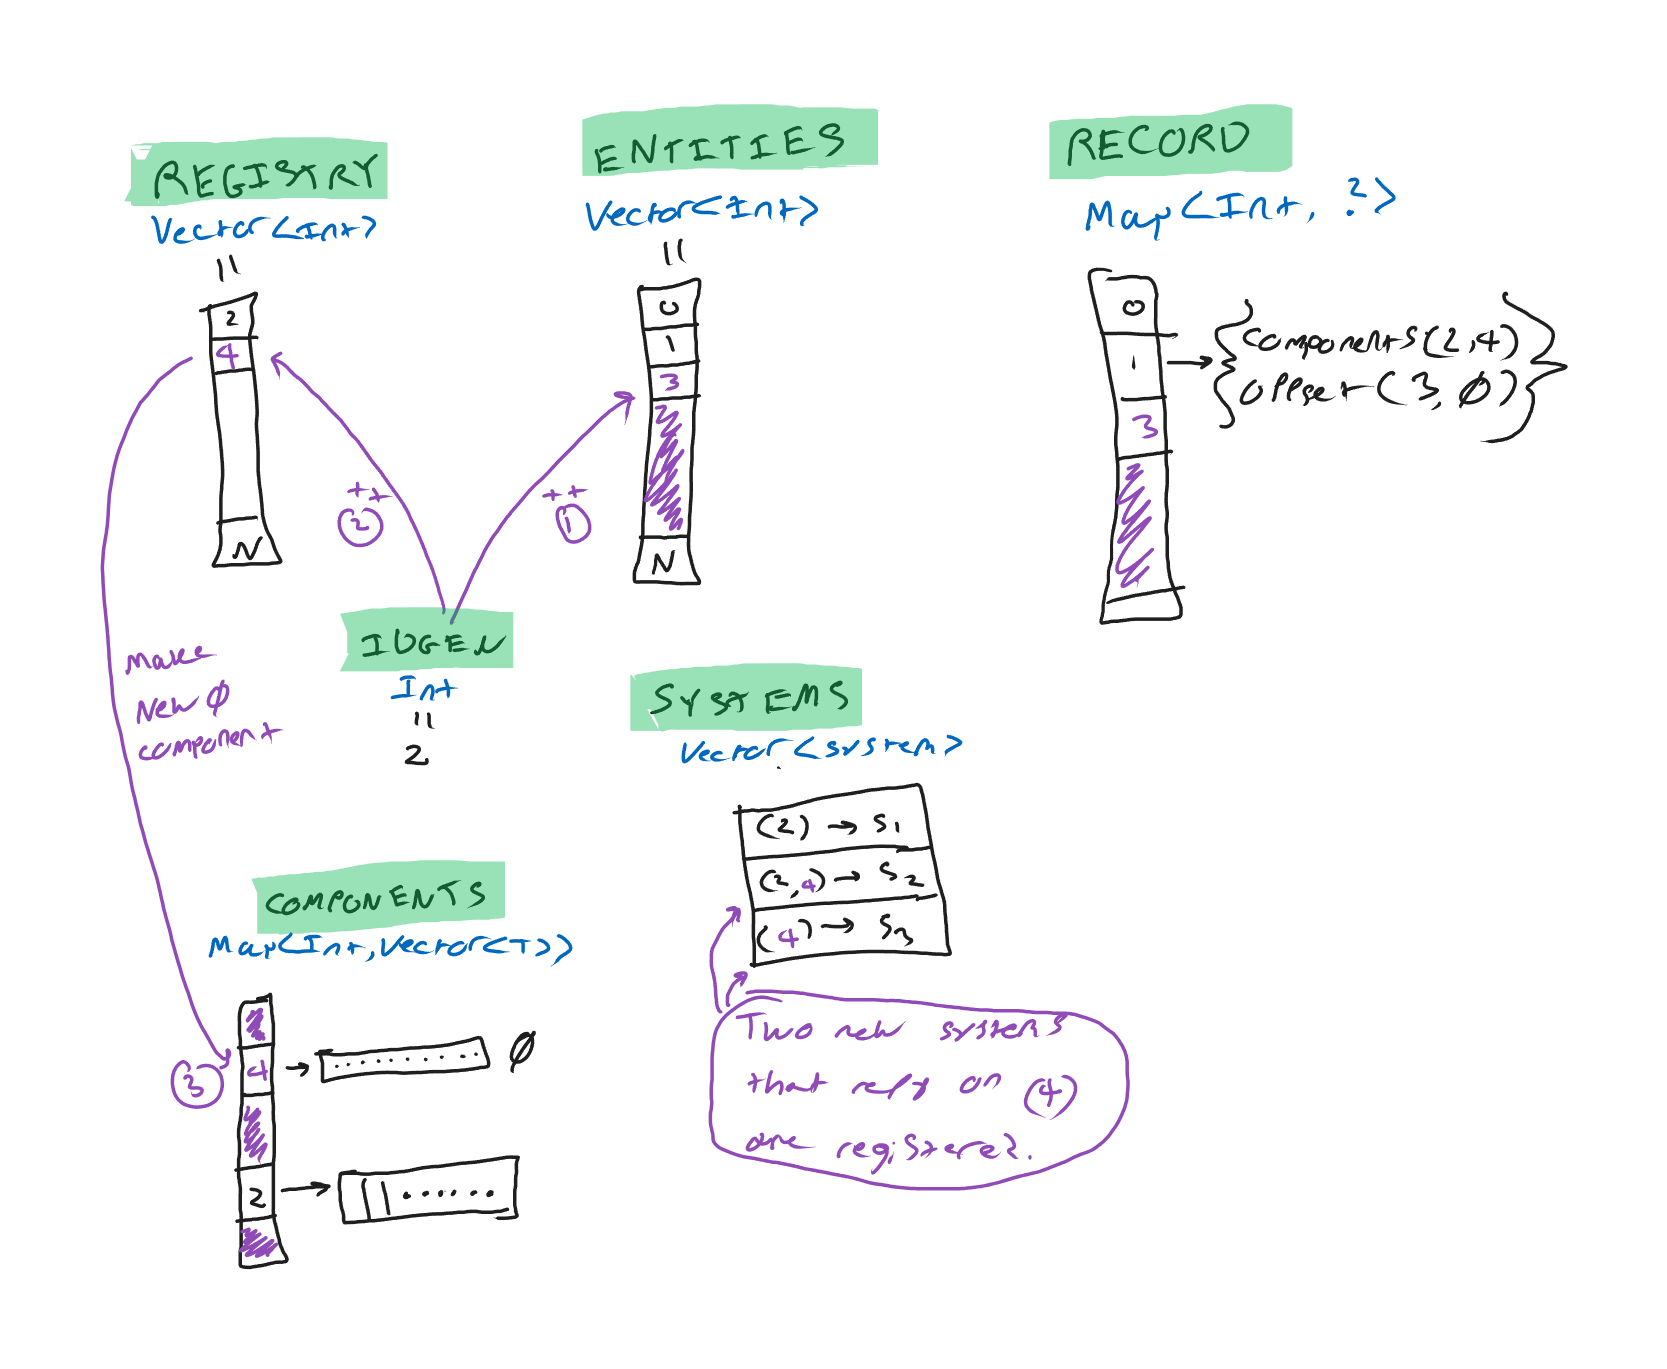
\includegraphics[width=0.5\linewidth]{resources/naive_ecs.png}
    \caption{Basic ECS Architecture Adding New Component}
    \label{fig:naive_ecs}
\end{figure}


There are a total of 6 major components to consider in this ECS model. 

\subsubsection{Entity}
The entity part is emulated via a variable IDGEN which is shared to generate unique identifiers for components and entities. This global variable is incremented each time an entity or component is generated. The list of active entities, stored in ENTITIES, is a list of uint64\_t values generated by IDGEN. 

\begin{figure}[H]
    \centering
    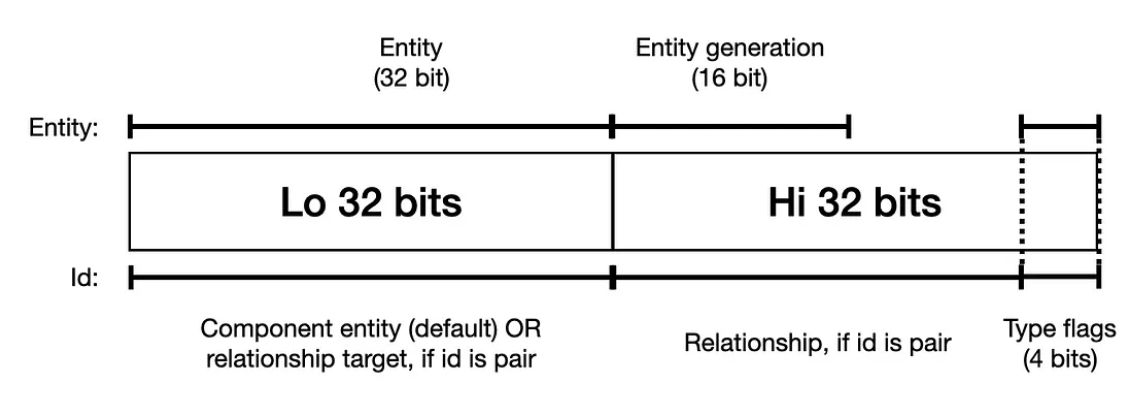
\includegraphics[width=0.5\linewidth]{resources/entity_generation.png}
    \caption{Smart Entity Generation in FLECS}
    \label{fig:entity_generation}
\end{figure}

% https://ajmmertens.medium.com/doing-a-lot-with-a-little-ecs-identifiers-25a72bd2647
Later in the paper, there will be mentions of a popular ECS framework called FLECS \textnormal{(Fast Lightweight Entitiy Component System)}. FLECS is unique in that it makes their ID generator more intelligent to decrease query times and grant the ability to define components at runtime with a technique called runtime tagging. The way IDs lower query times is by storing entity relationships inside the top half bits and the actual entity id in the lower half. The same technique is used to create entities with empty components, also known as tags, to the ID.  

\subsubsection{Component}
Similar to ENTITIES, the list of unique components is stored in the REGISTRY. The REGISTRY contains ID's that can be used as keys to access the COMPONENTS map. The COMPONENTS map then map's unique component ID's to homogenous component data. 

\subsubsection{System}
Systems can be registered to the SYSTEMS vector by providing two arguments: the set of components to iterate on and a function pointer to initiate the system. When the ECS world progresses by 1 tick, each system will have ran once.

\subsubsection{From Entitiy \textrightarrow{} Component}
In order to load the components of a given entity, the RECORD map is used. This map keeps track of the positions of components inside a homogenous component vector. Although this may be the case, a keen observer may notice how much more lookup is needed to load a single entity versus an entire component. \\

In order to load a specific entity, the ECS must:

\begin{enumerate}
    \item Check the Entity RECORD.
    \item Load the following components in COMPONENTS.
    \item Load the offsets in each component.
    \item Return to user.
\end{enumerate}

In order to load a specific component:

\begin{enumerate}
    \item Load the registery.
    \item Load the following component.
    \item Return to user.
\end{enumerate}

% TODO: source
This instinctively feels like a heavy tradeoff but in real-time simulations it's unlikely that there will be more direct entity queries versus batch component queries.


\subsubsection{System Queries}
An important detail is omitted from this diagram: the way a system queries for entities and components. This detail is omitted in this example because the structure is simple enough to hand query abilities directly to the developer. Since this example only runs in single threaded contexts there is no need to overcomplicate it.

% https://github.com/SanderMertens/ecs-faq
\subsection{Existing ECS And Implementation Styles}
As shown in the previous section, the definition of an ECS gives many different ways to implement it into an architecture. The following are a brief overview of different ECS architectures seen in various real implementions. The concurrent model this paper proposes falls under the category of a Dense ECS.  

\subsubsection{Dense ECS}
\begin{figure}[htbp]
    \centering
    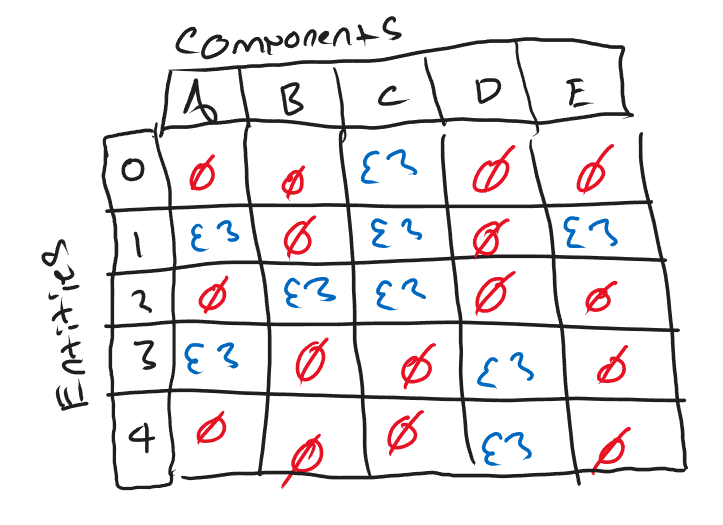
\includegraphics[width=0.5\linewidth]{resources/dense_ecs.png}
    \caption{Dense ECS Architecture Example}
    \label{fig:dense_ecs}
\end{figure}

A dense ECS stores entities in tables, where components are columns and entities are rows. This gives way for fast queries and easy to iterate over. Some popular examples of this type of ECS is FLECS and Unity's own ECS, Unity DOTS.

\subsubsection{Sparse ECS}
% https://programmingpraxis.com/2012/03/09/sparse-sets/
% https://citeseerx.ist.psu.edu/viewdoc/summary?doi=10.1.1.30.7319
% https://research.swtch.com/sparse 
Before discussing sparse ECS architectures, a small introduction into sparse sets is necessary. They are a datastructure dedicated to keeping the invariance of the following property:
\begin{equation*}
    \forall v \in \{0,\ldots, n-1\} : \text{D}[S[v]] = v
\end{equation*}
In the property above, $D$ and $S$ represent two vectors. The dense vector and sparse vector respectively. By using these two vectors in unison: lookup, insertion, and deletion time are all $O(1)$ and iteration is $O(n)$. 

% https://skypjack.github.io/2019-03-21-ecs-baf-part-2-insights/
% TODO: source https://www.flecs.dev/flecs/md_docs_2FAQ.html#:~:text=When%20you%20are%20comparing%20Flecs,queries%20are%20faster%20in%20Flecs
% https://github.com/SanderMertens/ecs-faq?tab=readme-ov-file
The main advantage of the sparse ECS is how fast it is to teest if an entity contains a component. Because of this, sparse ECS's advantages come in the form of query optimization. In a sparse ECS, a query iterates over all entities with the first queried for component, then takes that set and tests each subsequent component if every entity has it. Bitset ECS's are known to use similar approaches in their implementations.

Sparse sets also have another use where systems own their own sparse sets and they are kept to date each tick during runtime. These system owned sparse sets are then used to collect entities related to the system. An example of an ECS that does this technique is ecst. 

Overall, it's important to know that sparse set ECS's are popular in situations where fast add/remove of single component operations are preferred over efficient batch operations. To back this claim, FLECS which is a popular dense ECS published its own benchmarking data against other wide-industry used ECS's. From their data, FLECS has slower add/remove operations then EnTT, a popular sparse set based ECS. Regardless of the advantages and disadvantages of using sparse vs dense ECS's, it can be summed up nicely by the creator of EnTT:

\begin{quote}
    \textbf{It’s a matter of taste}, in fact.
        - Michele Caini
\end{quote}

\subsubsection{Bitset-based}
A bitset-based ECS stores components in arrays such that the entity id is emulated as the index. It then uses a bitset to indicate which components an entity has in table where the index is the entity. Some examples of bitset implementations are EntityX and Specs.

\subsubsection{Reactive}
A reactive ECS is more different than the others in this list. A reactive ECS uses signals emitted from mutating entities to keep individual lists of which entities belong to which system. Entitas is an example of this. 

\subsection{Concurrency in ECS Implementations}
The majority of ECS implementations I investigated had trivial or very basic concurrency support.
% https://github.com/SanderMertens/flecs/issues/281

The example of one I did find was that of FLECS. The concurrency model in FLECS is simple. The user initally sets the amount of worker threads manually, and entities matched with a system will be divided equally across threads. 
This system is not ideal because performance is left at the table. If the model allowed for individual read/write permissions the engine could open up to more performance gains.
 
